\chapter{Membuat Aplikasi Akademik Sederhana dari Oracle APEX Online}
\section{Membuat tabel dan data yang diperlukan yang sudah dinormalisasi  }
\par
\begin{enumerate}
    \item Hal pertama yang perlu dilakukan adalah masuk ke Microsoft Excel, dan buat tabel mahasiswa, dosen, kuliah, nilai dan jadwal dan data-datanya.
    \begin{figure}[!htbp]
\centering
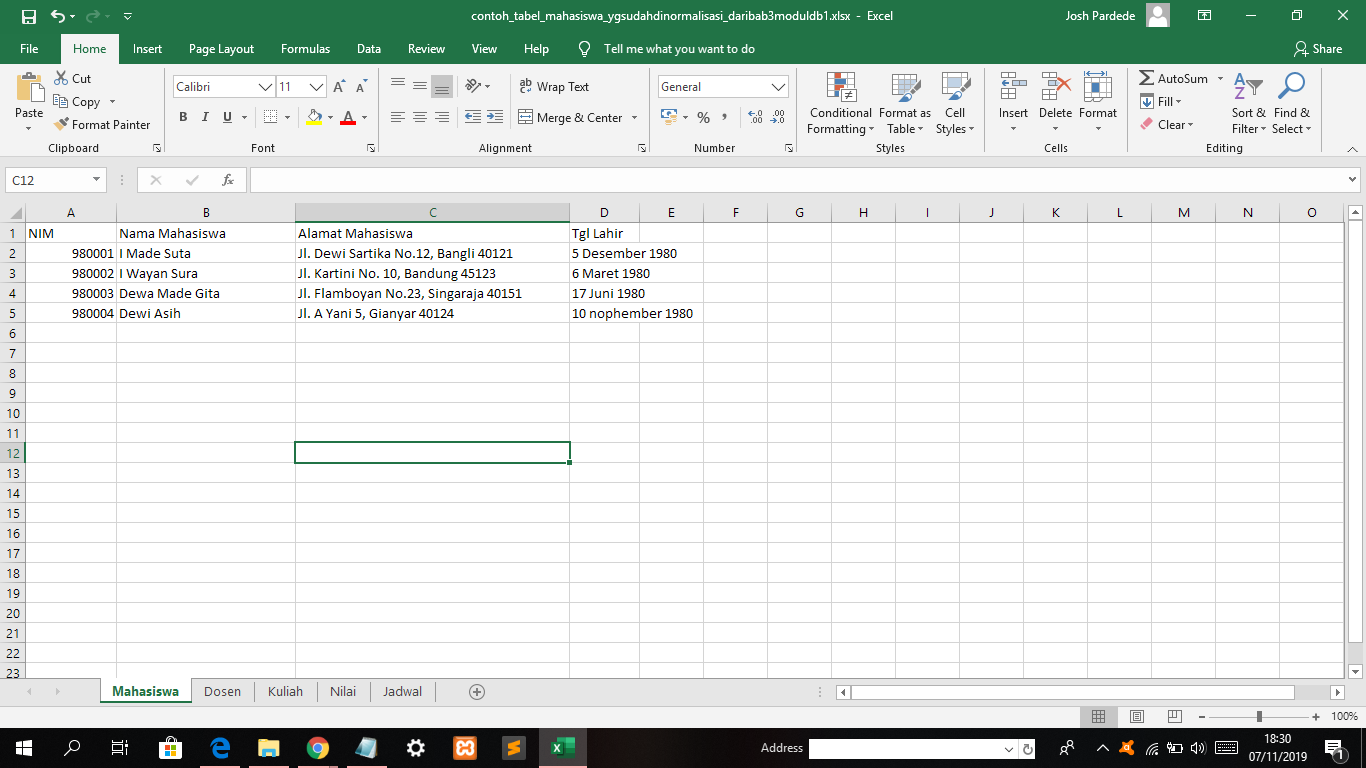
\includegraphics[width=10cm,height=9cm]{figures/1tabel_mahasiswa.png}
\caption{Tabel Mahasiswa}
\label{penanda}
\end{figure}
    
\begin{figure}[!htbp]
\centering
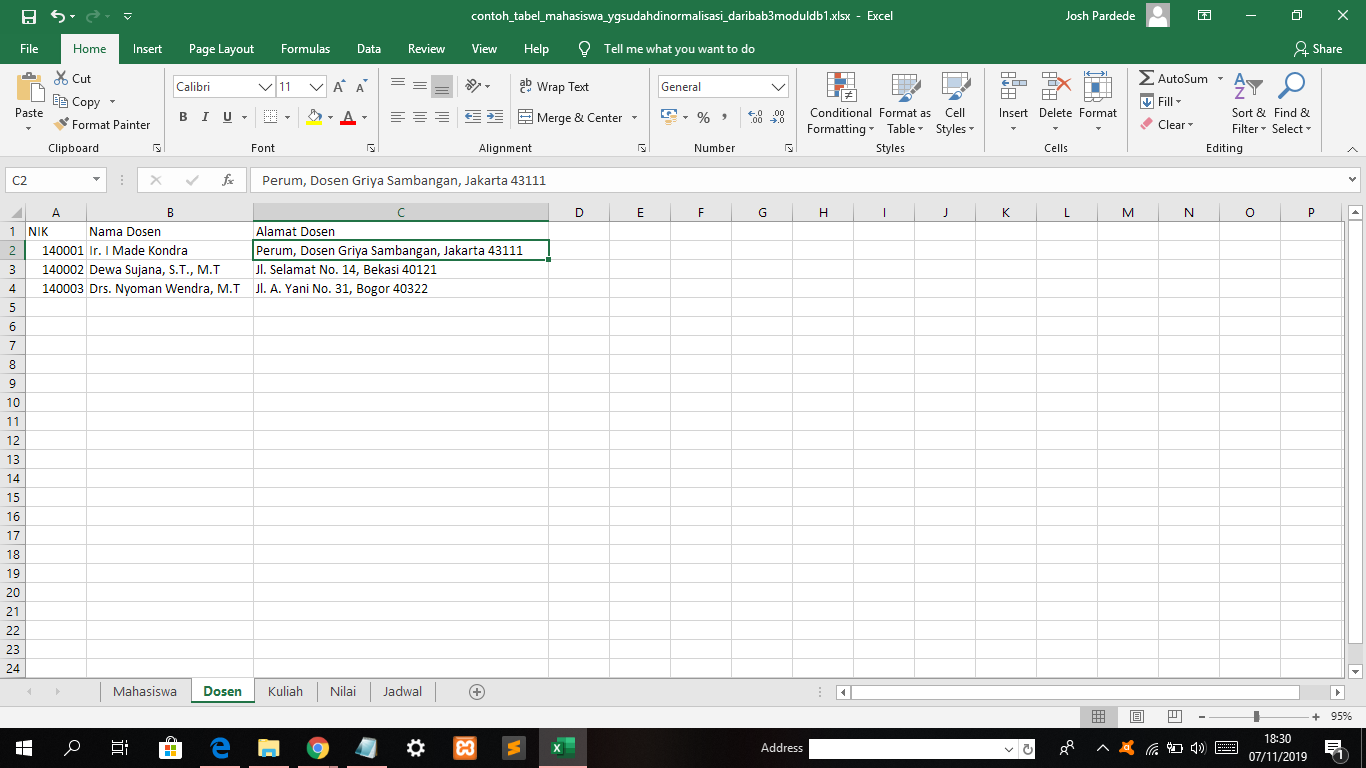
\includegraphics[width=11cm,height=9cm]{figures/2tabel_dosen.png}
\caption{Tabel Dosen}
\label{penanda}
\end{figure}
    
\begin{figure}[!htbp]
\centering
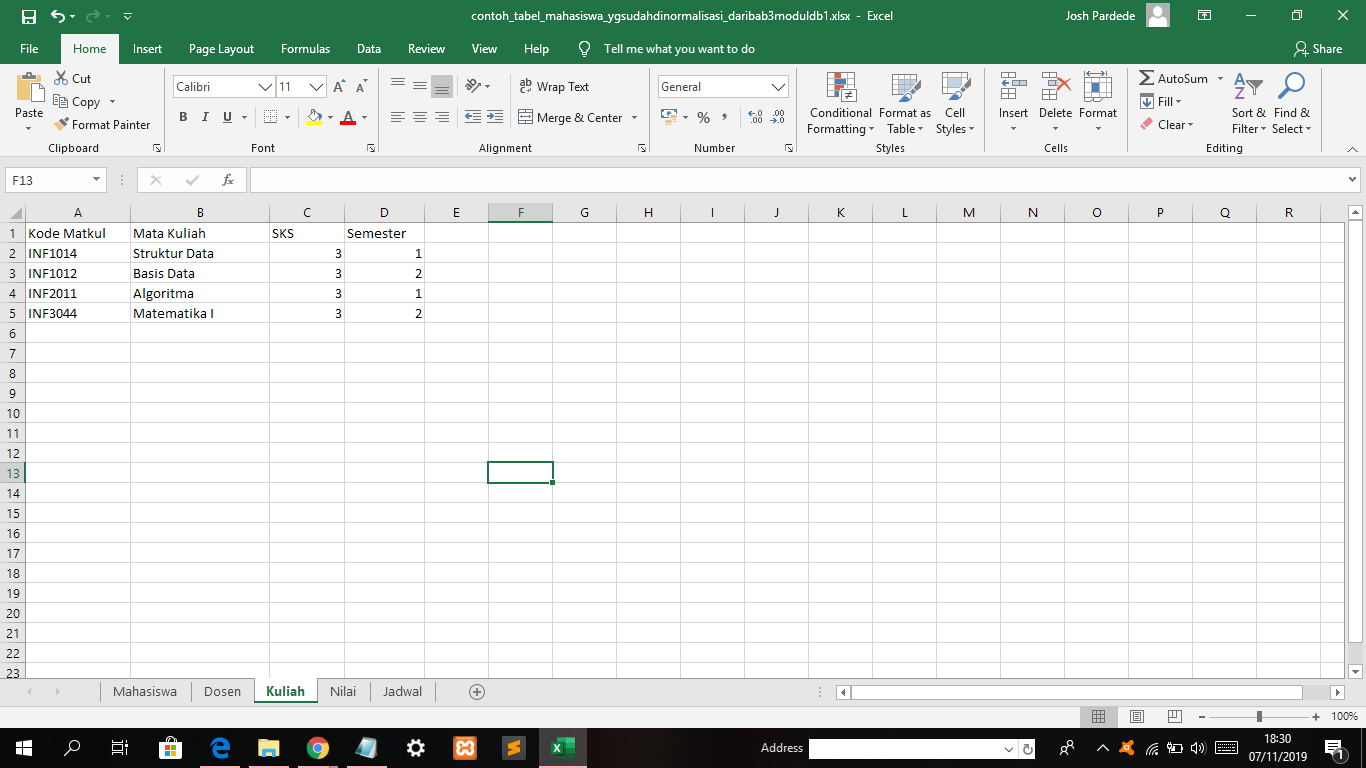
\includegraphics[width=11cm,height=9cm]{figures/3tabel_kuliah.png}
\caption{Tabel Kuliah}
\label{penanda}
\end{figure}
    
\begin{figure}[!htbp]
\centering
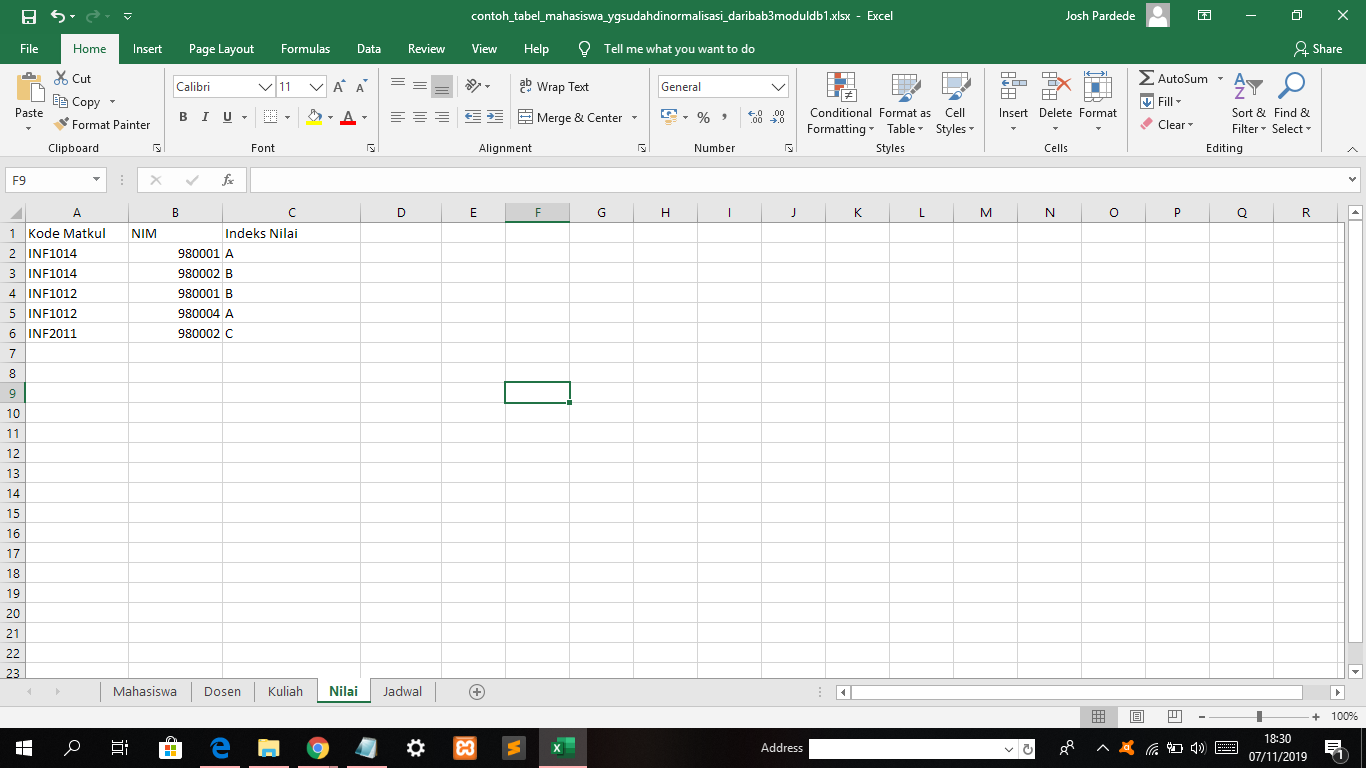
\includegraphics[width=10cm,height=8cm]{figures/4tabel_nilai.png}
\caption{Tabel Nilai}
\label{penanda}
\end{figure}

\begin{figure}[!htbp]
\centering
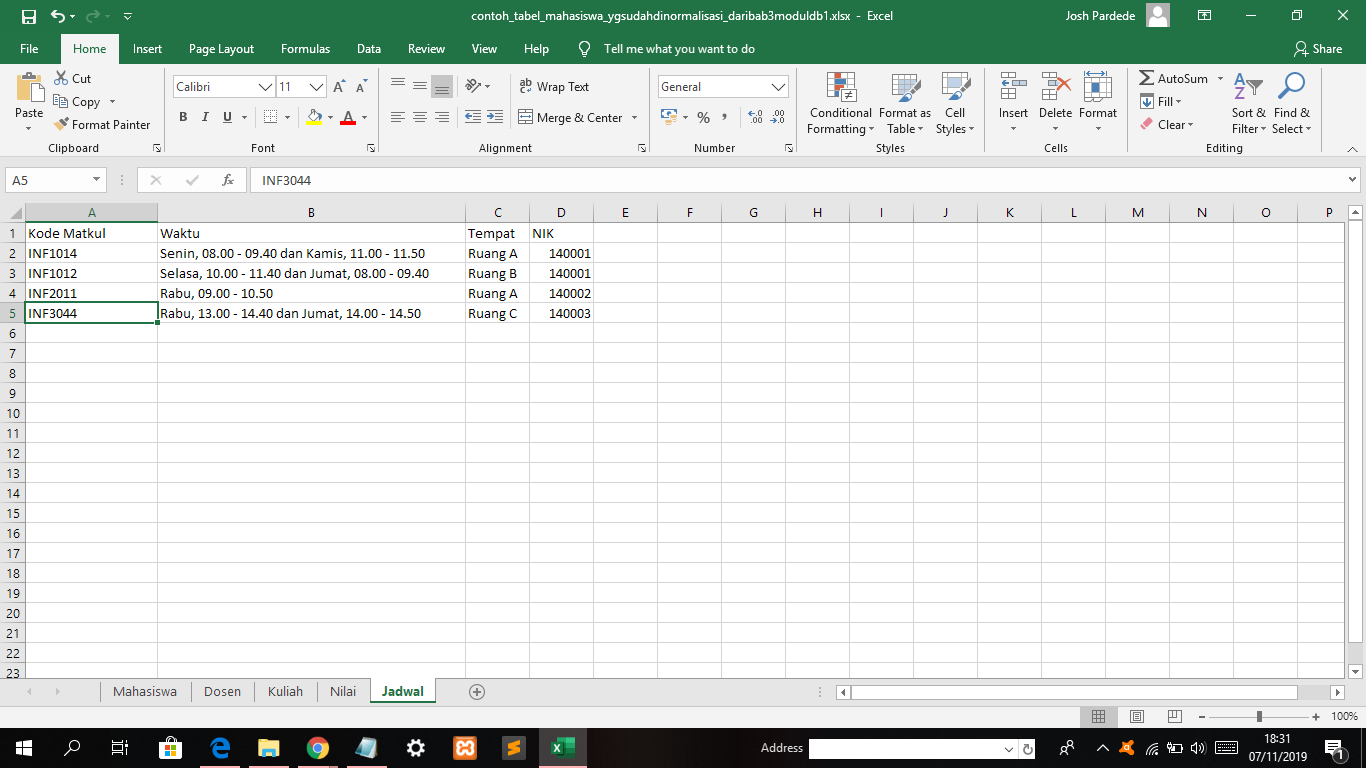
\includegraphics[width=10cm,height=8cm]{figures/5tabel_jadwal.png}
\caption{Tabel Jadwal}
\label{penanda}
\end{figure}

\item Setelah itu, Masuk ke website Oracle Apex dan masuk ke workspace yang sudah ada. Masuk ke Appbulider.

\begin{figure}[!htbp]
\centering
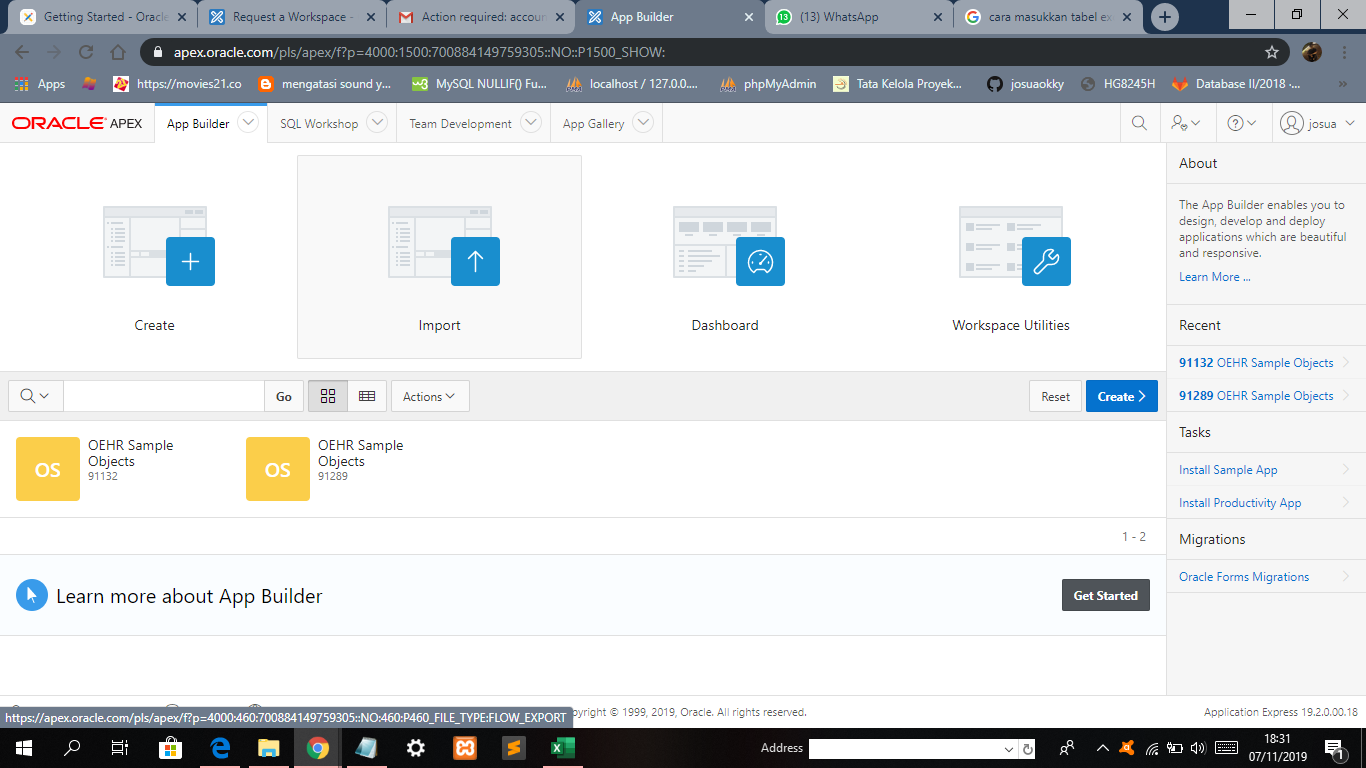
\includegraphics[width=10cm,height=8cm]{figures/6appbuilder.png}
\caption{App Builder}
\label{penanda}
\end{figure}

\item Pilih create.

\begin{figure}[!htbp]
\centering
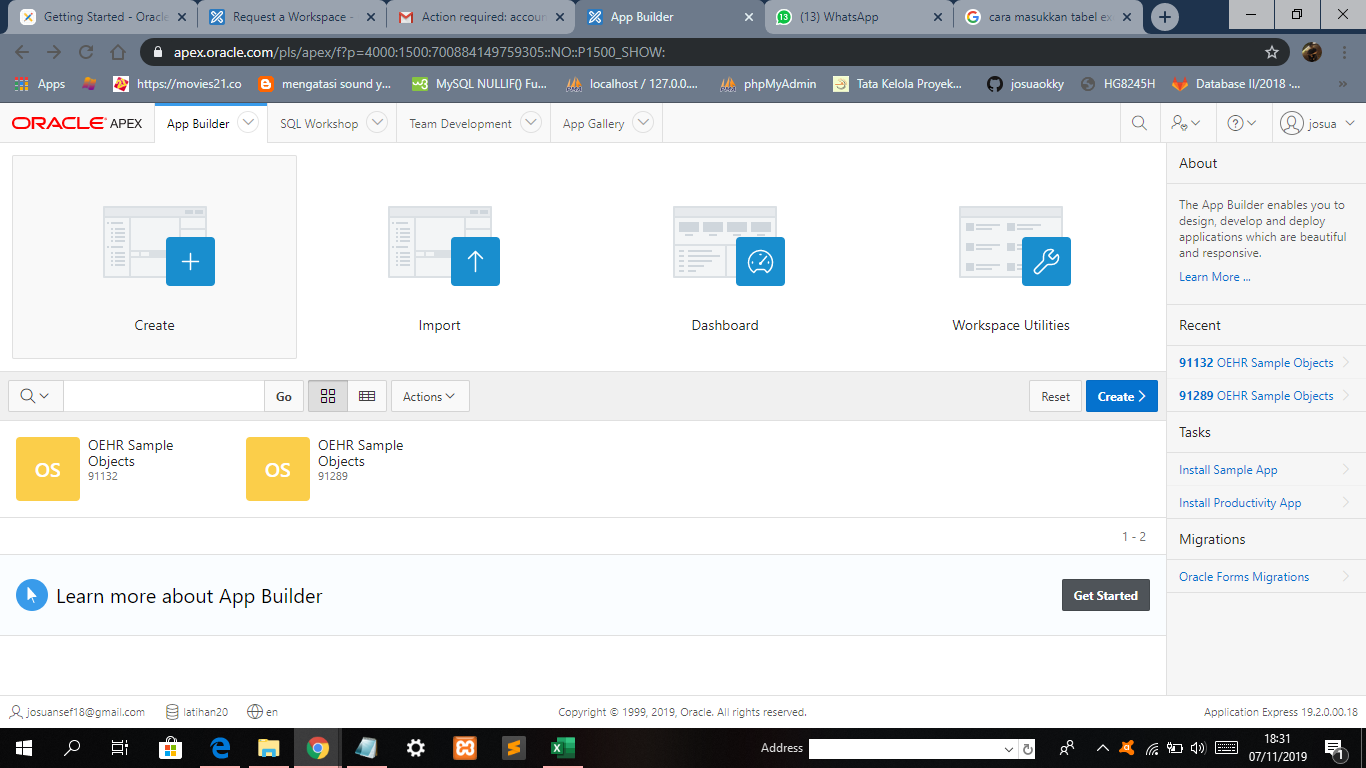
\includegraphics[width=10cm,height=7cm]{figures/7create.png}
\caption{Create}
\label{penanda}
\end{figure}

\item Selanjutnya, pilih from a file.

\begin{figure}[!htbp]
\centering
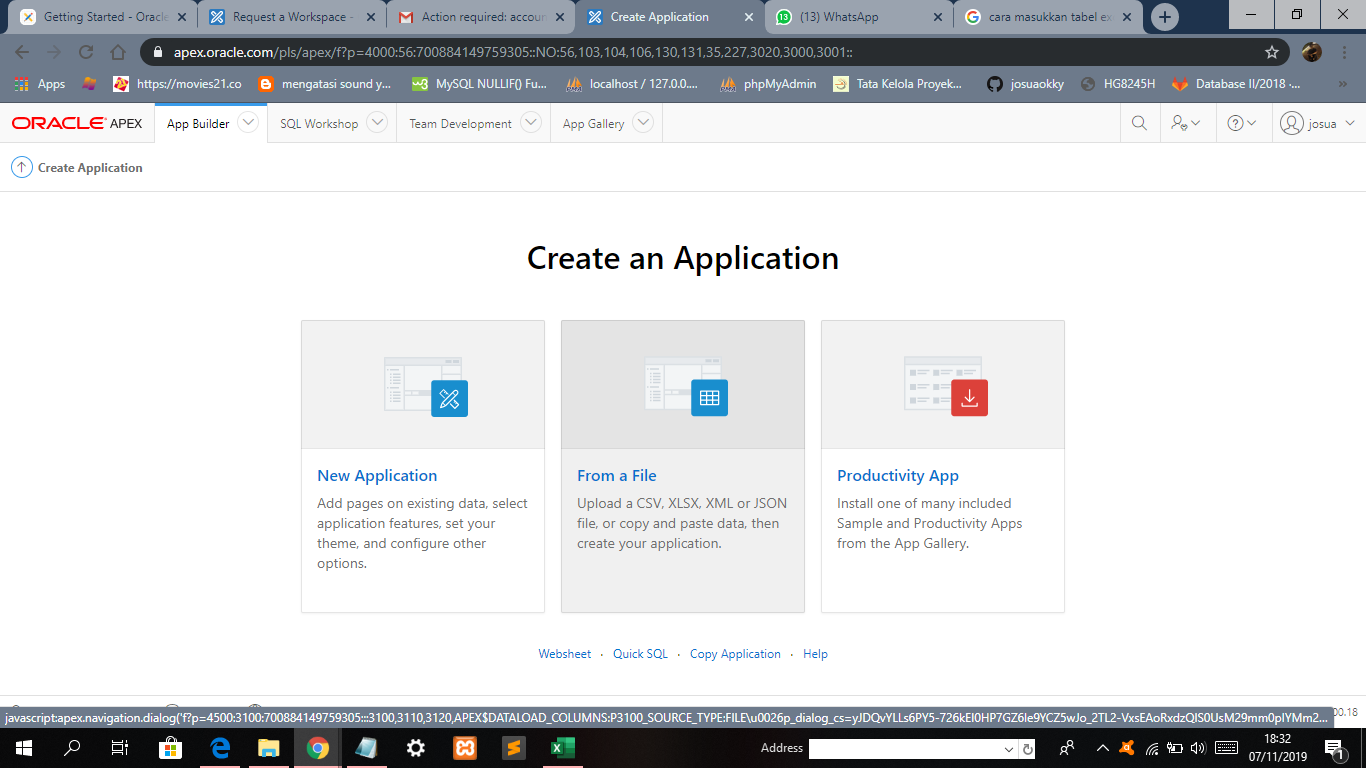
\includegraphics[width=10cm,height=8cm]{figures/8fromafile.png}
\caption{From a File}
\label{penanda}
\end{figure}

\item Pilih Choose File dan cari file xlsx (excel) yang didalamnya ada tabel-tabel yang diperlukan.

\begin{figure}[!htbp]
\centering
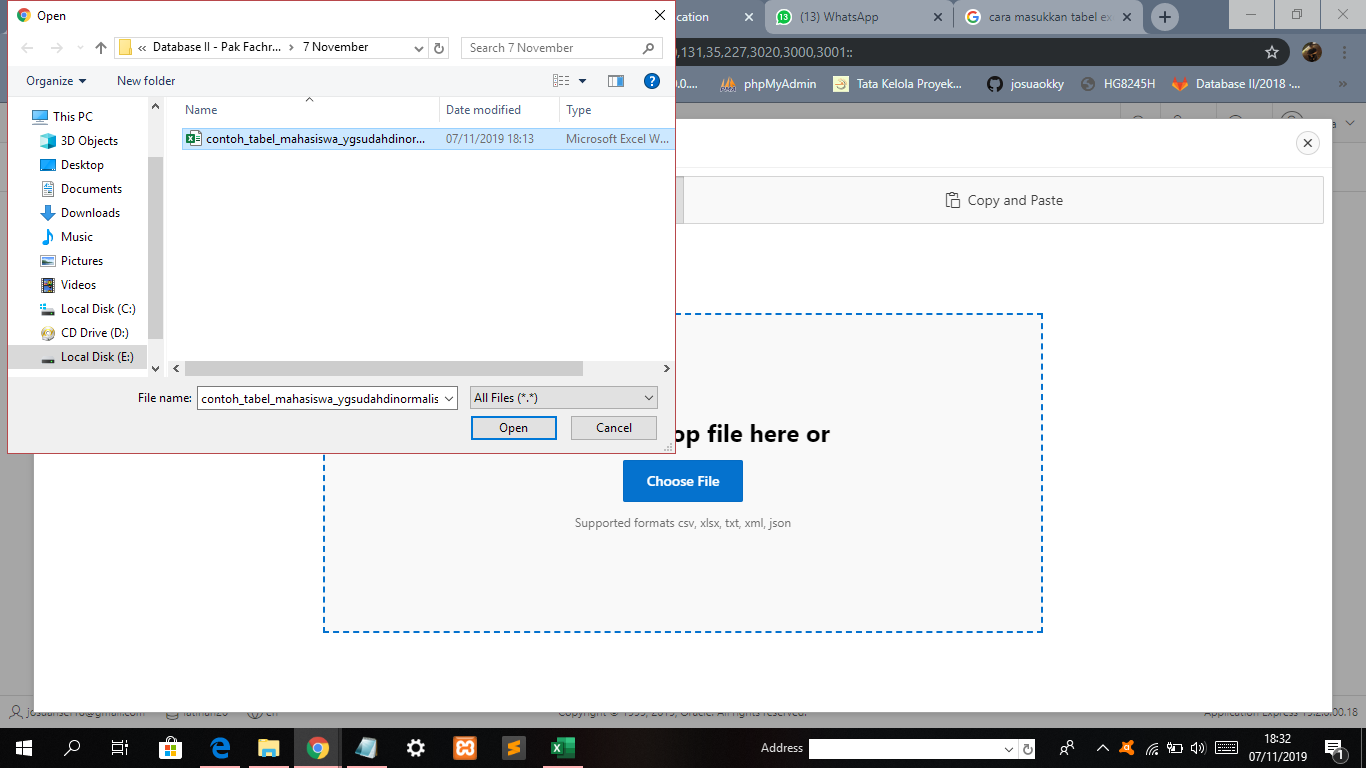
\includegraphics[width=11cm,height=7cm]{figures/9choosefile.png}
\caption{Choose File}
\label{penanda}
\end{figure}

\item Selanjutnya masukkan Table Name-nya : MAHASISWA dan select sheet : Mahasiswa Lakukan load data pada tabel mahasiswa. Begitu juga dengan tabel Dosen, tabel Kuliah, tabel Nilai dan tabel Jadwal

\begin{figure}[!htbp]
\centering
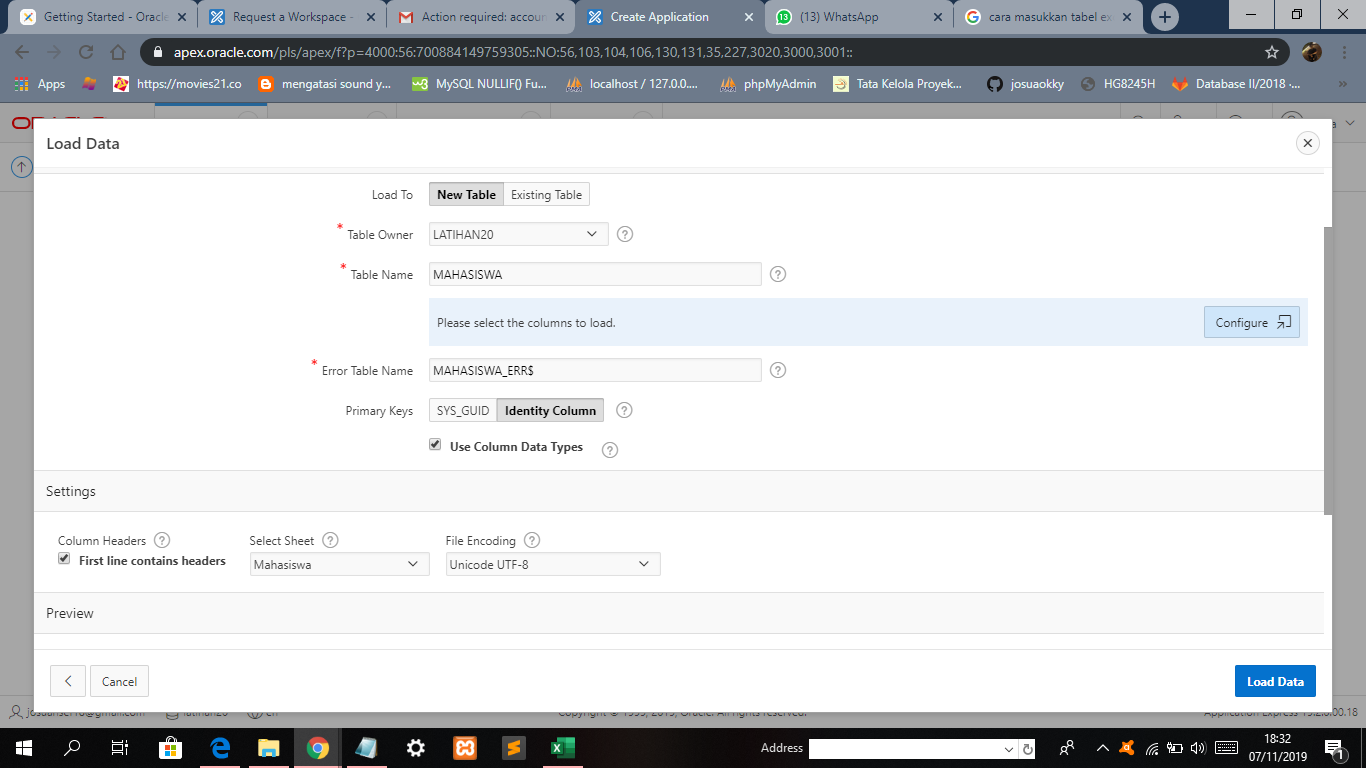
\includegraphics[width=11cm,height=8cm]{figures/10loadmahasiswa.png}
\caption{Load Mahasiswa}
\label{penanda}
\end{figure}

\begin{figure}[!htbp]
\centering
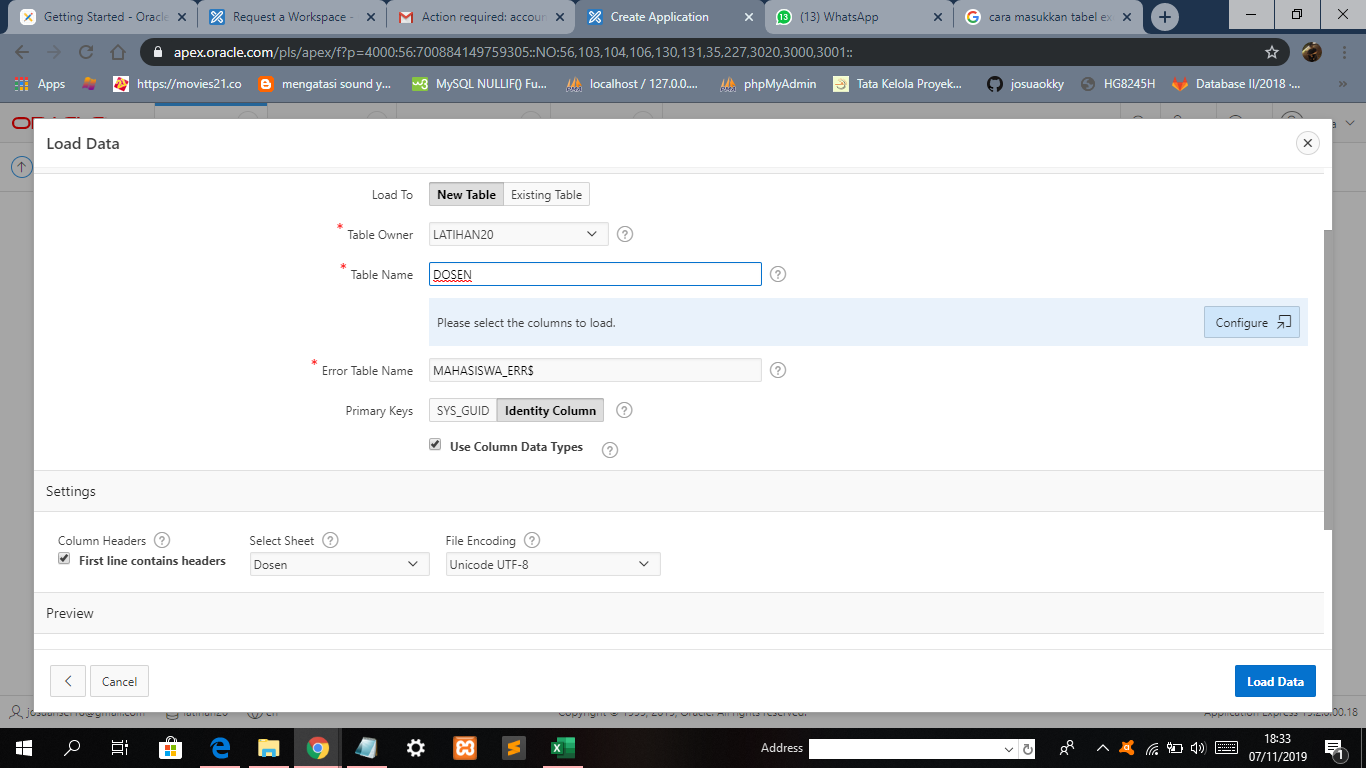
\includegraphics[width=10cm,height=8cm]{figures/11loaddosen.png}
\caption{Load Dosen}
\label{penanda}
\end{figure}

\begin{figure}[!htbp]
\centering
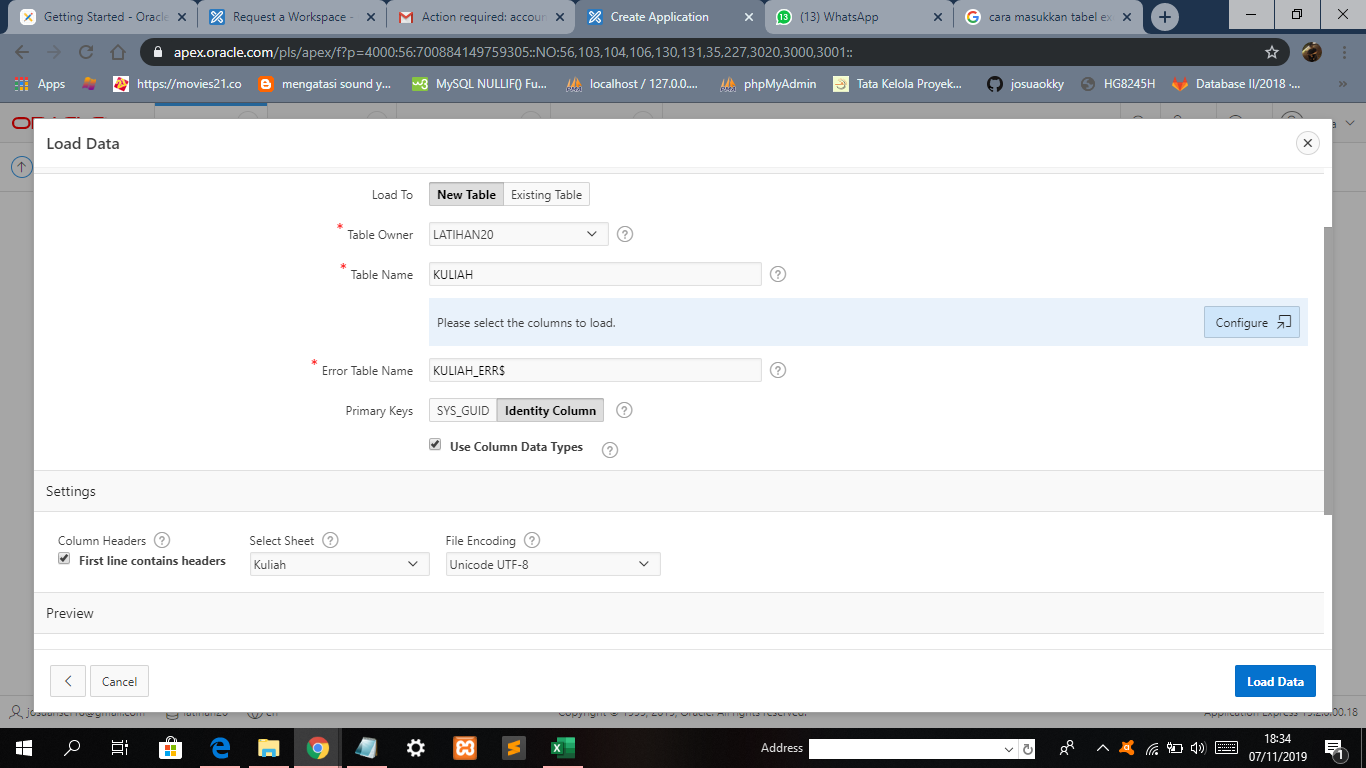
\includegraphics[width=10cm,height=8cm]{figures/12loadkuliah.png}
\caption{Load Kuliah}
\label{penanda}
\end{figure}

\begin{figure}[!htbp]
\centering
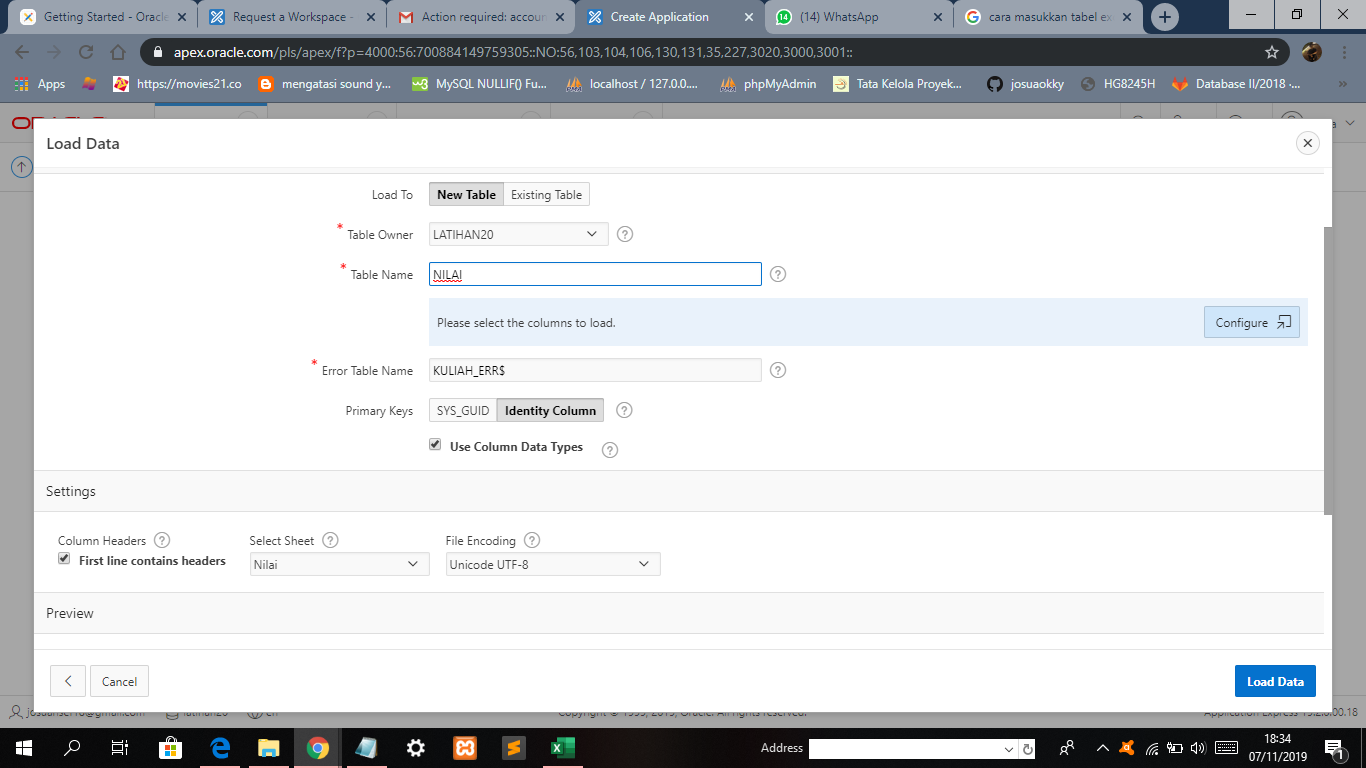
\includegraphics[width=10cm,height=8cm]{figures/13loadnilai.png}
\caption{Load Nilai}
\label{penanda}
\end{figure}

\begin{figure}[!htbp]
\centering
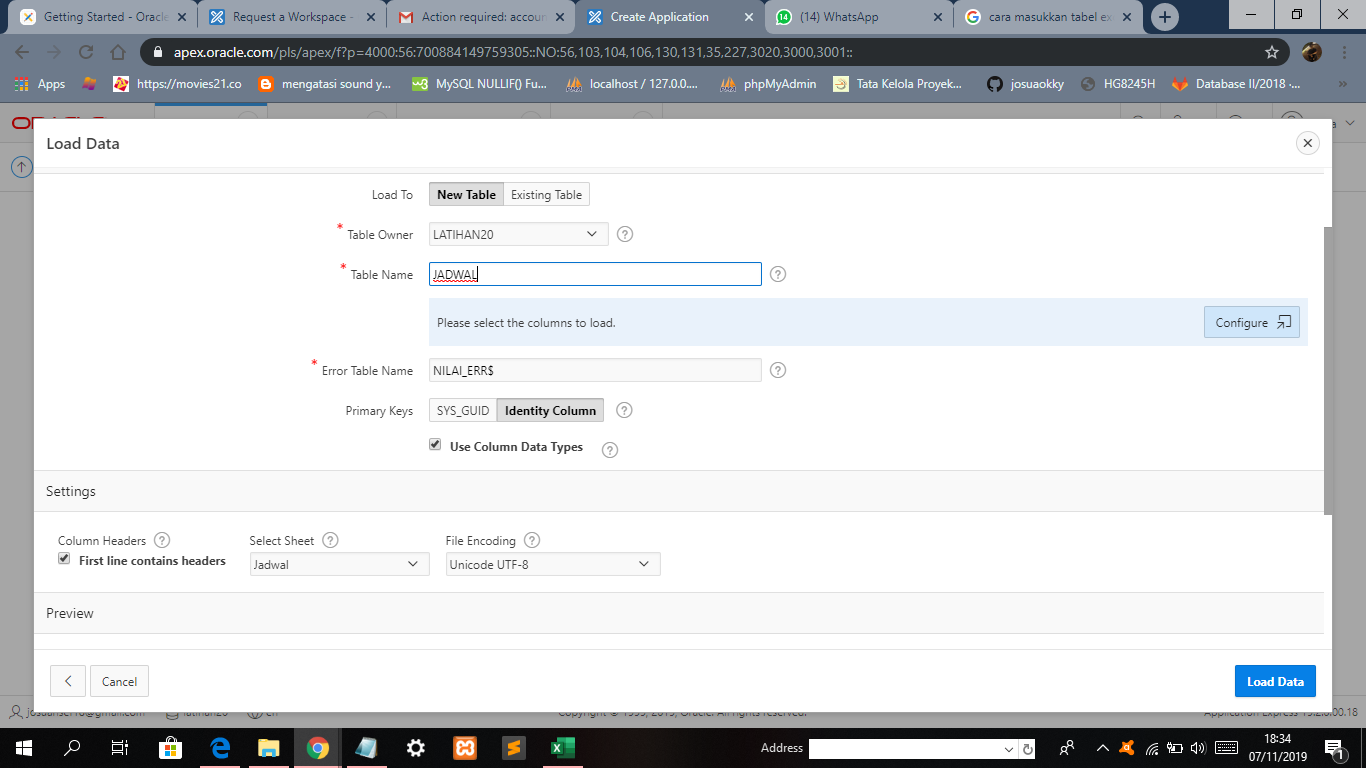
\includegraphics[width=10cm,height=8cm]{figures/14loadjadwal.png}
\caption{Load Jadwal}
\label{penanda}
\end{figure}

\item Setelah melakukan load data pada setiap tabe, kembali ke halaman SQL Workshop
\begin{figure}[!htbp]
\centering
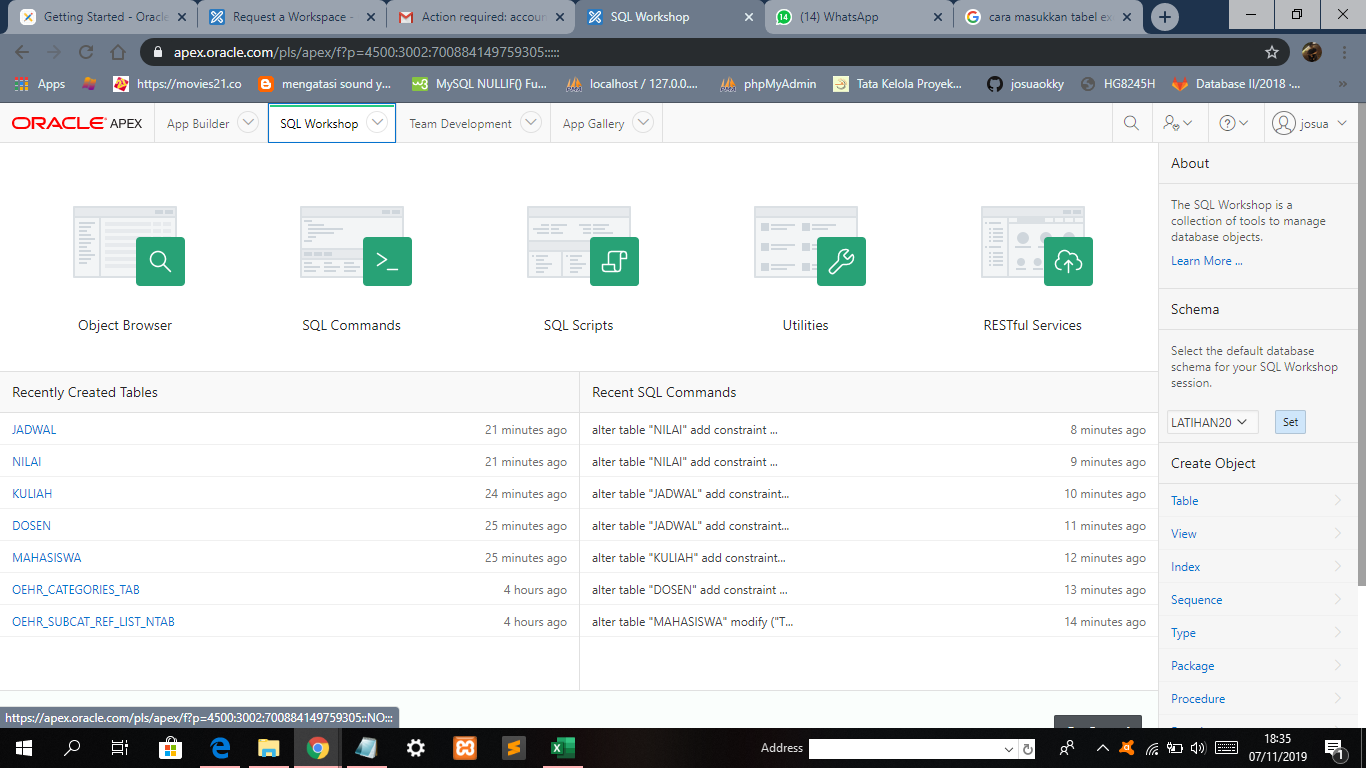
\includegraphics[width=10cm,height=8cm]{figures/15sqlworkshop.png}
\caption{SQL Workshop}
\label{penanda}
\end{figure}

\item Setelah itu, pilih/ klik tabel MAHASISWA pada tampilan menu sebelah kiri layar. Selanjutnya pada Kolom Constraint Type, pilih Primary Key untuk membuat primary key pada tabel MAHASISWA. Berikutnya pada Primary Key Column 1, pilih NIM(NUMBER) untuk memilih properti tabel yang ingin dijadikan primary key, yaitu properti yang bisa menampung data yang unik.
\\ Lakukan hal yang sama pada tabel DOSEN, KULIAH

\begin{figure}[!htbp]
\centering
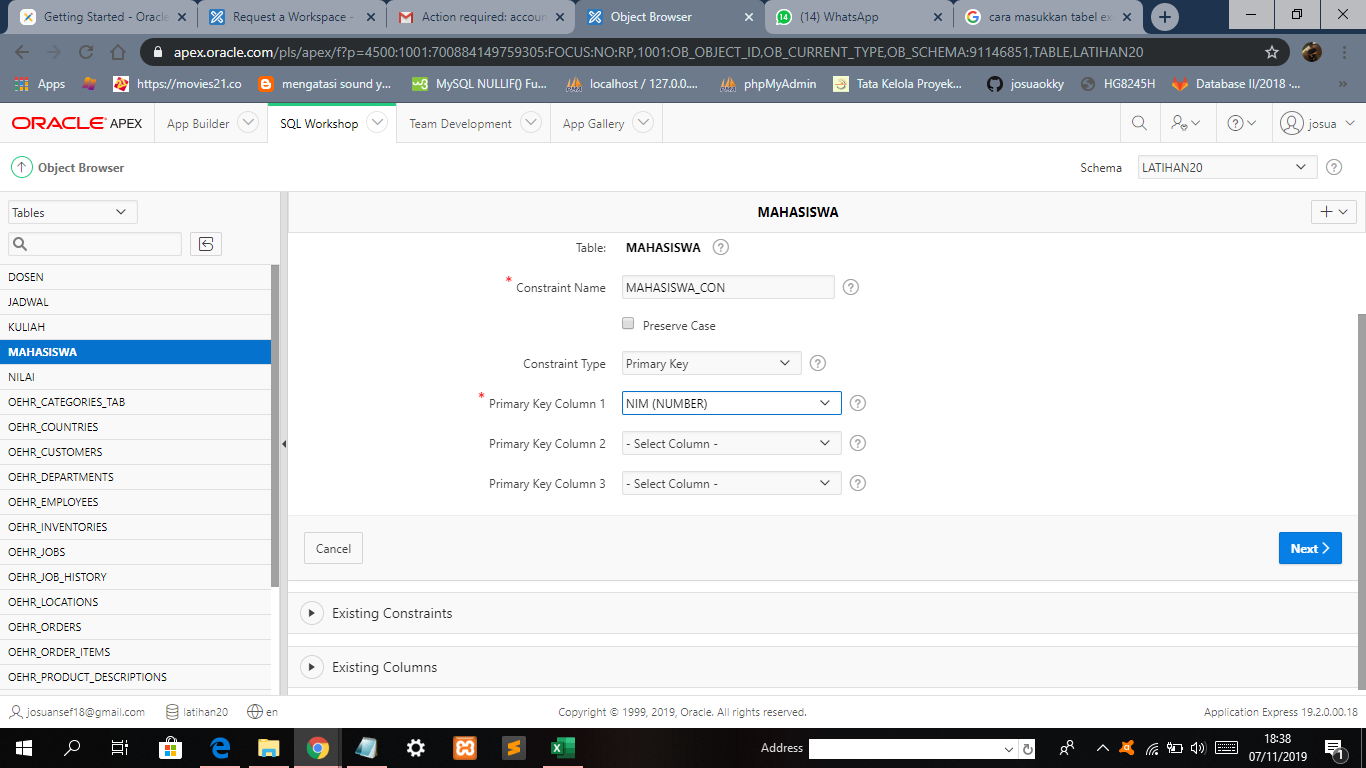
\includegraphics[width=10cm,height=8cm]{figures/16primary_mahasiswa.png}
\caption{Primary Key Mahasiswa}
\label{penanda}
\end{figure}

\begin{figure}[!htbp]
\centering
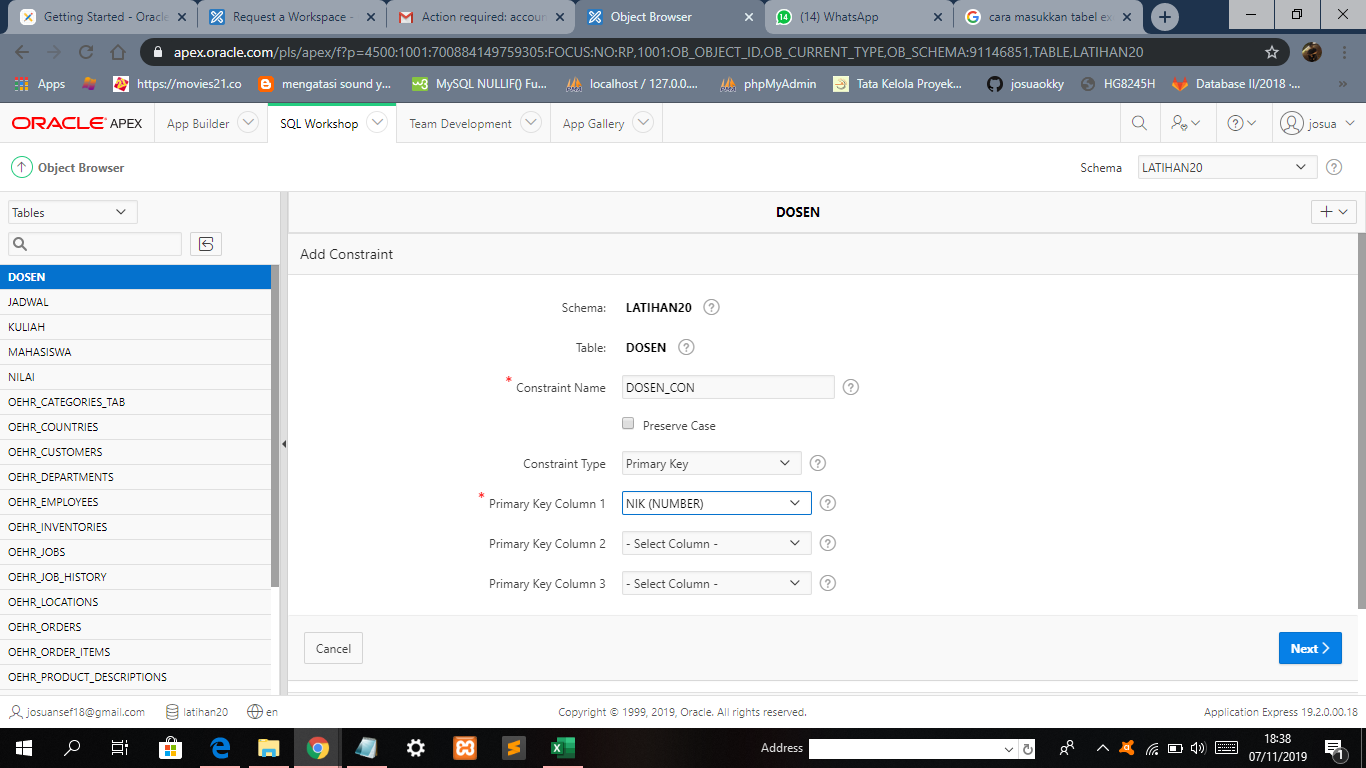
\includegraphics[width=10cm,height=8cm]{figures/17primary_dosen.png}
\caption{Primary Key Dosen}
\label{penanda}
\end{figure}

\begin{figure}[!htbp]
\centering
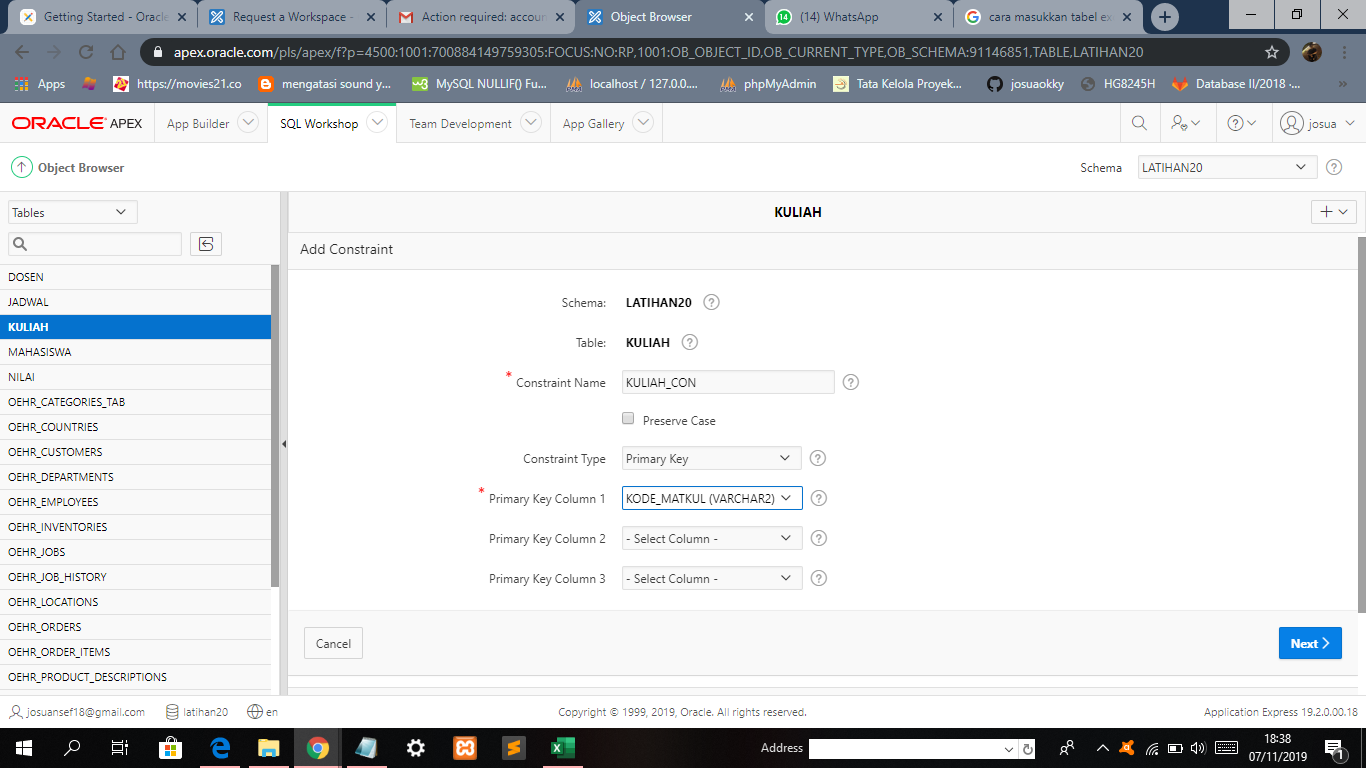
\includegraphics[width=10cm,height=8cm]{figures/18primary_kuliah.png}
\caption{Primary Key Kuliah}
\label{penanda}
\end{figure}

\item  Jika sudah membuat primary key pada tiga tabel tersebut, selanjutnya kita akan membuat foreign key dari tabel NILAI dan JADWAL.

\\
Pada saat membuat foreign key tabel NILAI, klik dua kali KODE MATKUL dan  pada Reference Table Name, pilih tabel yang mempunyai relasi KODE MATKUL dengan tabel NILAI , yaitu tabel KULIAH.
\\
Begitu juga NIM. Lakukan lagi hal yang sama dengan NIM, lalu pilih tabel yang mempunyai relasi NIM dengan tabel NILAI, yaitu tabel MAHASISWA.

\begin{figure}[!htbp]
\centering
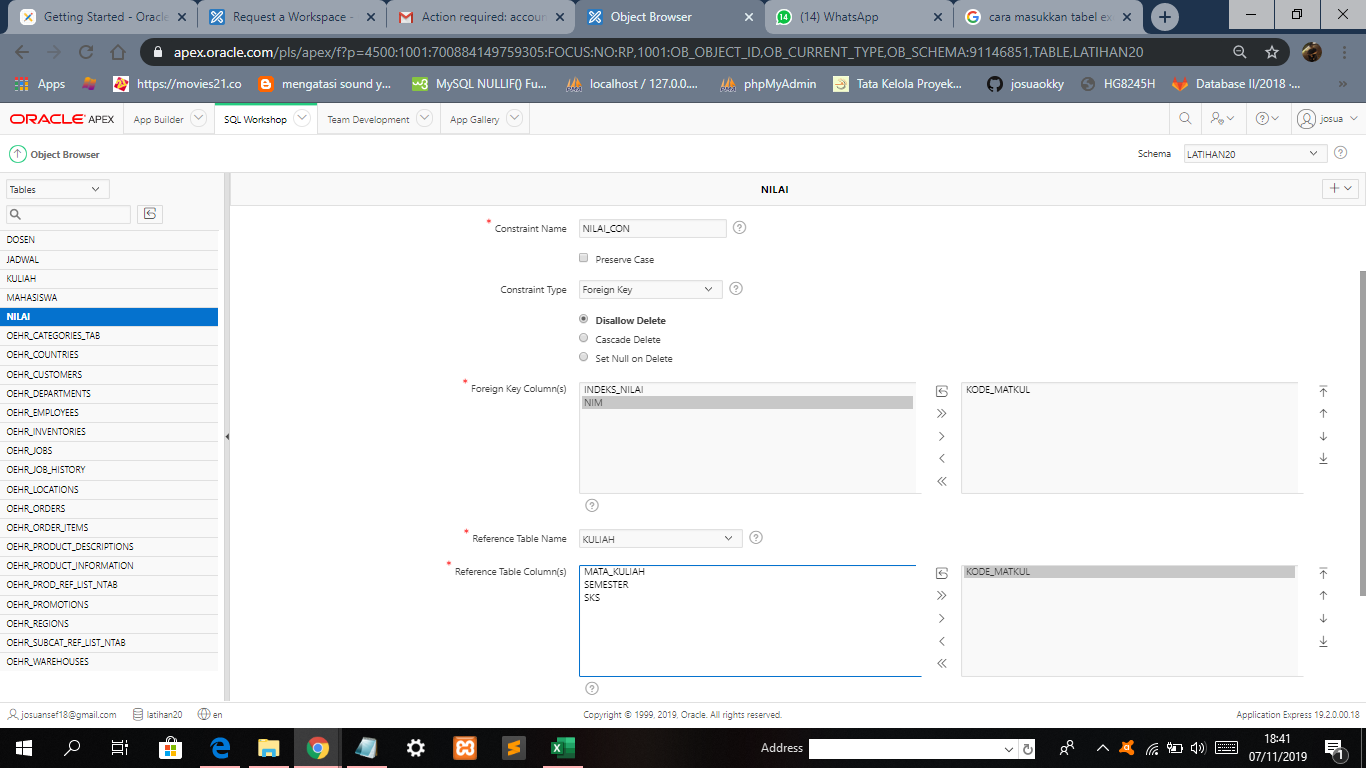
\includegraphics[width=10cm,height=8cm]{figures/19foreign_nilai.png}
\caption{Foreign KODE_MATKUL pada tabel NILAI}
\label{penanda}
\end{figure}

\begin{figure}[!htbp]
\centering
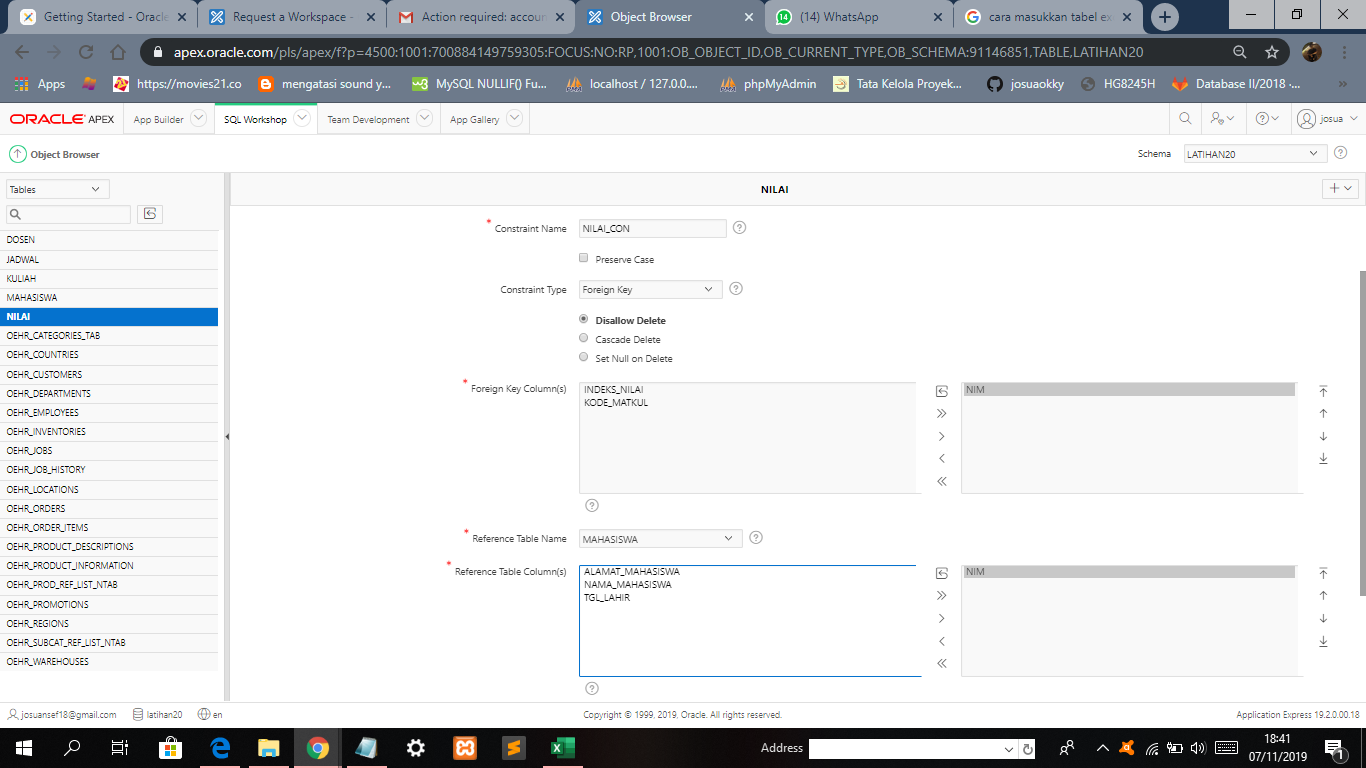
\includegraphics[width=10cm,height=8cm]{figures/20foreign_nilai1.png}
\caption{Foreign NIM pada tabel NILAI}
\label{penanda}
\end{figure}



\item Selanjutnya, buat foreign key pada tabel JADWAL, klik dua kali KODE MATKUL dan  pada Reference Table Name, pilih tabel yang mempunyai relasi KODE MATKUL dengan tabel NILAI , yaitu tabel KULIAH.
\\
Begitu juga NIK. Lakukan lagi hal yang sama dengan NIK, lalu pilih tabel yang mempunyai relasi NIK dengan tabel NILAI, yaitu tabel DOSEN.

\begin{figure}[!htbp]
\centering
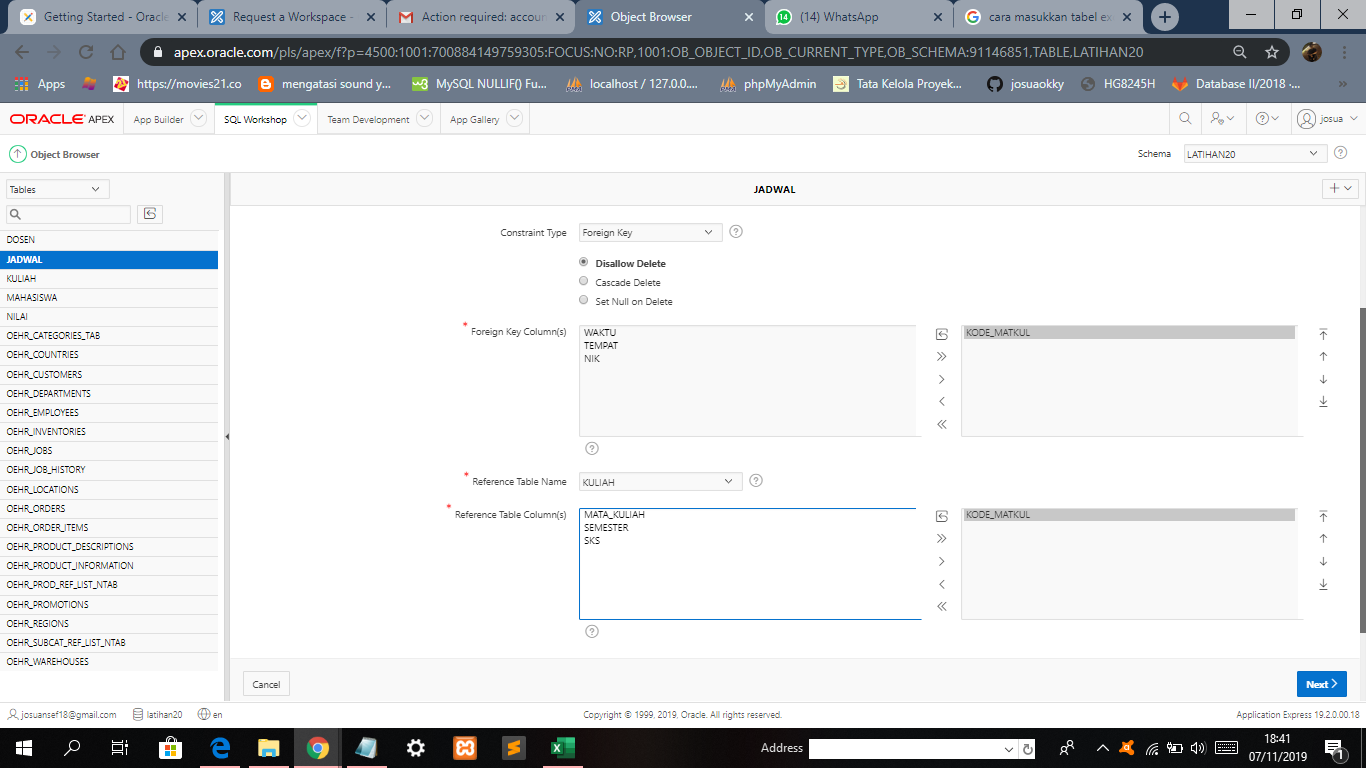
\includegraphics[width=10cm,height=7cm]{figures/21foreign_jadwal.png}
\caption{Foreign KODE_MATKUL pada tabel JADWAL}
\label{penanda}
\end{figure}

\begin{figure}[!htbp]
\centering
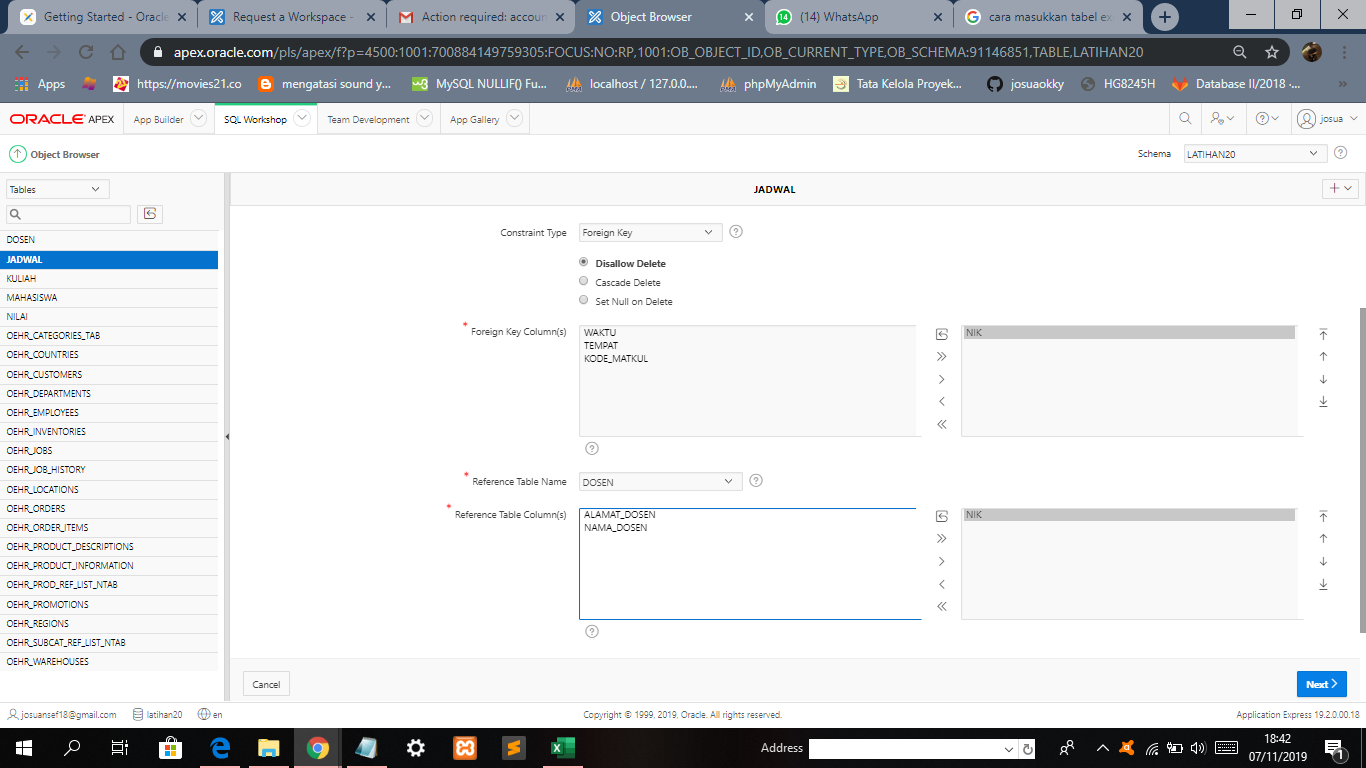
\includegraphics[width=10cm,height=7cm]{figures/22foreign_jadwal1.png}
\caption{Foreign NIK pada tabel JADWAL}
\label{penanda}
\end{figure}


\item Setelah membuat primary key dan foreign key pada pada setiap tabel, sekarang kembali ke App Builder.
\begin{figure}[!htbp]
\centering
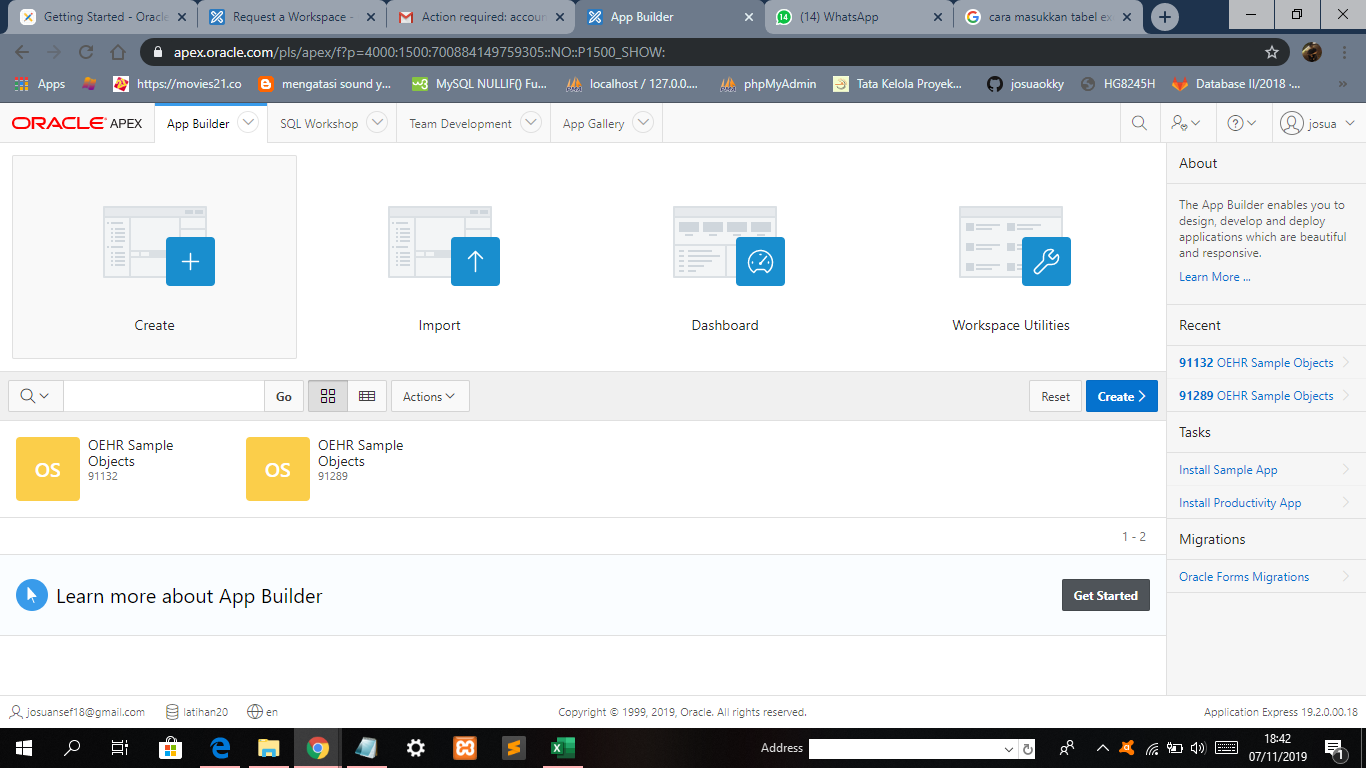
\includegraphics[width=10cm,height=7cm]{figures/23create_application.png}
\caption{App Builder}
\label{penanda}
\end{figure}
\item Pilih New Application.

\begin{figure}[!htbp]
\centering
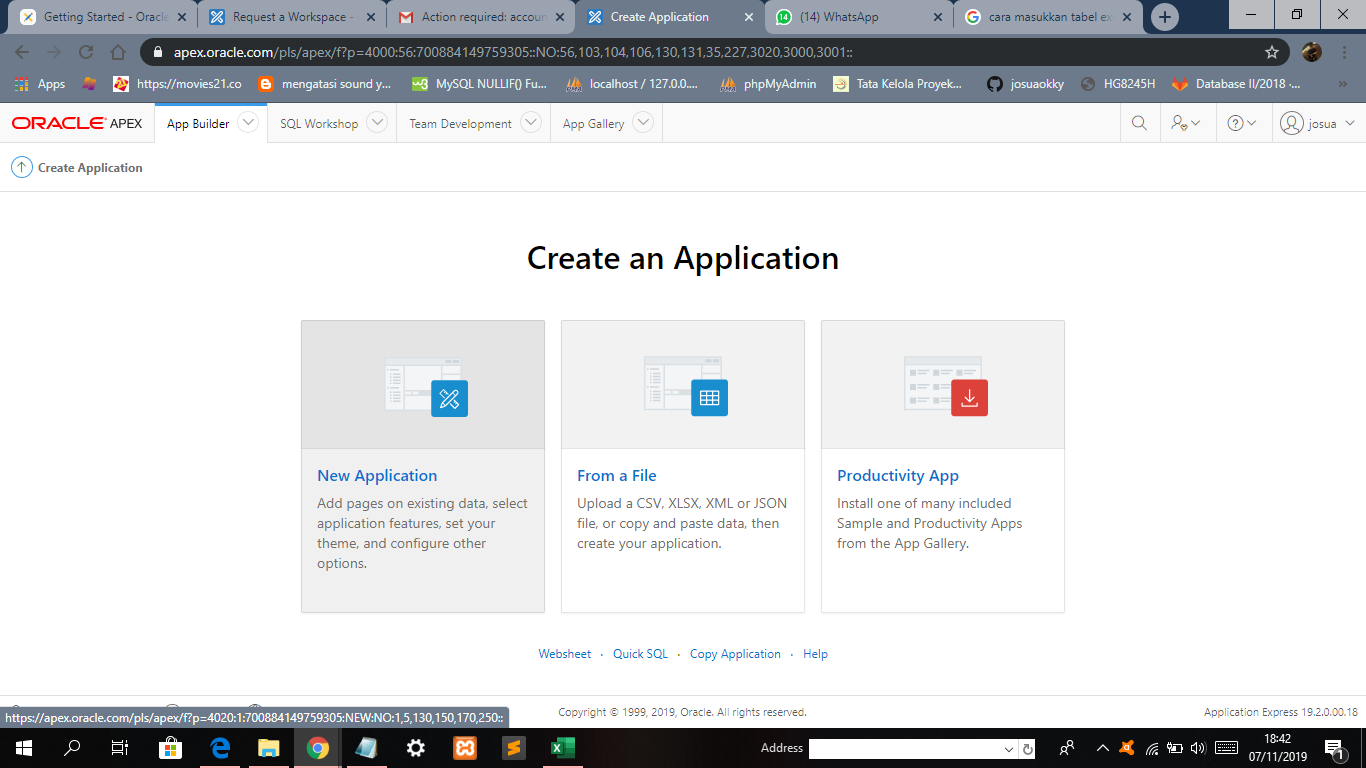
\includegraphics[width=10cm,height=7cm]{figures/24create_application.png}
\caption{Create Application}
\label{penanda}
\end{figure}

\item Buat nama aplikasinya, yaitu APLIKASI AKADEMIK SEDERHANA
\item Langkah selanjutnya adalah cara merelasikan dua tabel, yaitu kita mengketikkan query seperti gambar dibawah.
\begin{figure}[!htbp]
\centering
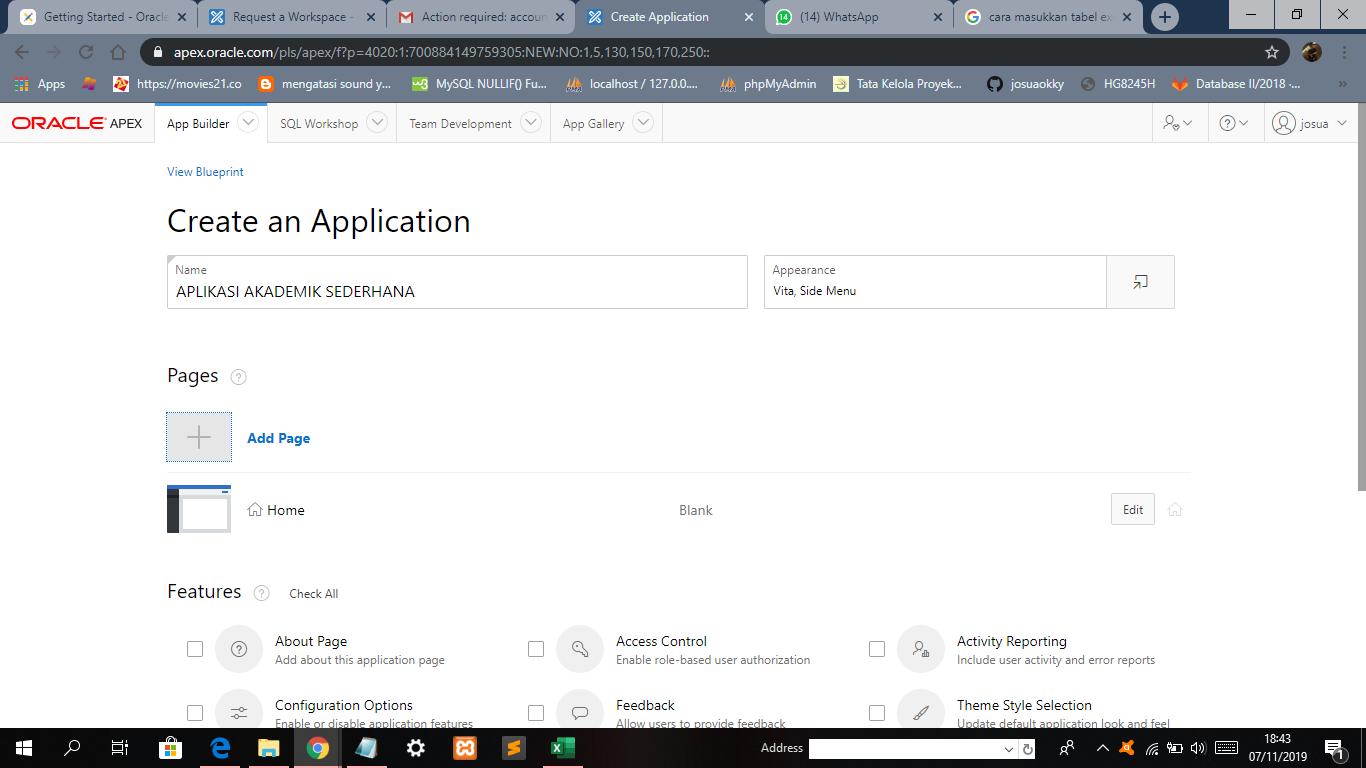
\includegraphics[width=10cm,height=7cm]{figures/25nama_aplikasi.png}
\caption{Nama Aplikasi}
\label{penanda}
\end{figure}

\item Klik Add Page, buat Page dengan nama MAHASISWA, DOSEN, KULIAH dan Dashboard. Tambah fitur fitur lainnya untuk melengkapi dan memperbanyak fitur pada aplikasi seperti Pages, dan fitur-fitur pada pages dan lain-lain.

\begin{figure}[!htbp]
\centering
\includegraphics[width=10cm,height=7cm]{figures/26add_pages.png}
\caption{Add Pages}
\label{penanda}
\end{figure}

\item Setelah itu, scroll ke bawah lalu klik Create Application.

\begin{figure}[!htbp]
\centering
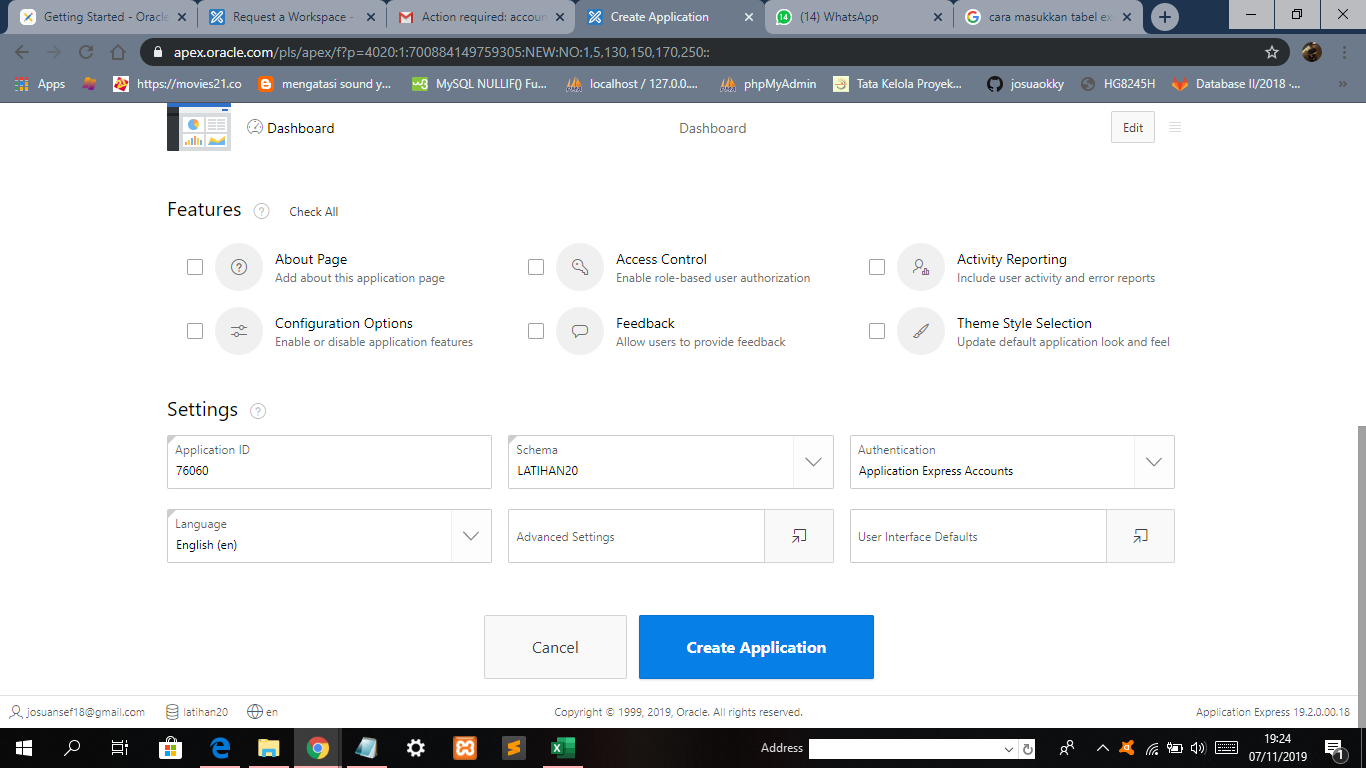
\includegraphics[width=10cm,height=7cm]{figures/30create_app.png}
\caption{Create Application}
\label{penanda}
\end{figure}

\item Selanjutnya setelah aplikasi telah suskses dibuat, pergi ke halaman App Builder dan klik Run Application.

\item  Setelah itu add page.
\begin{figure}[!htbp]
\centering
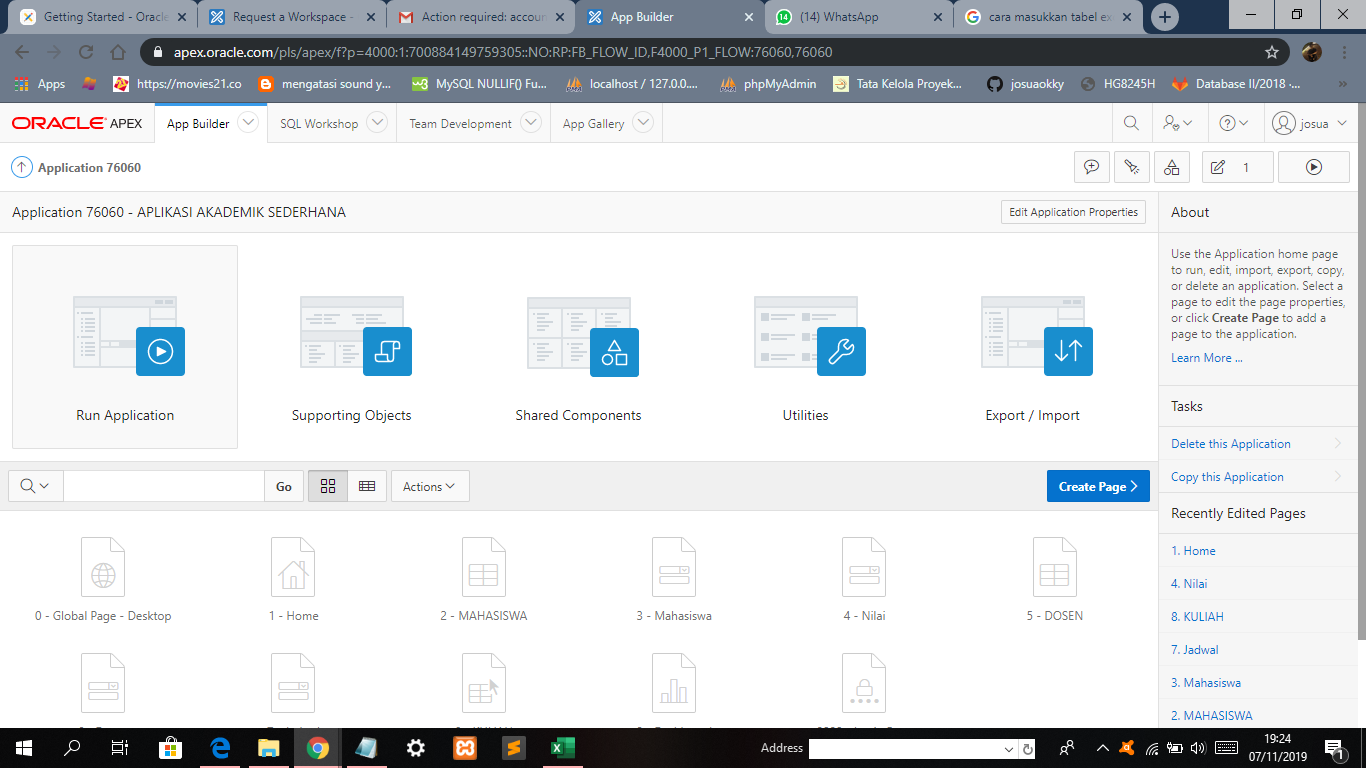
\includegraphics[width=10cm,height=7cm]{figures/31run.png}
\caption{Add page}
\label{penanda}
\end{figure}

\item Setelah itu, kita akan masuk ke halaman login aplikasi yang tadi baru dibuat. 
\\ Masuk ke link berikut {https://apex.oracle.com/pls/apex/f?p=76060:LOGIN_DESKTOP:706660752799964:::::} untuk login ke APLIKASI AKADEMIK SEDERHANA yang tadi baru dibuat. Masukkan :
\\ username : josuansef18@gmail.com
\\ password : Bandung2020

\item  Setelah itu add page.
\begin{figure}[!htbp]
\centering
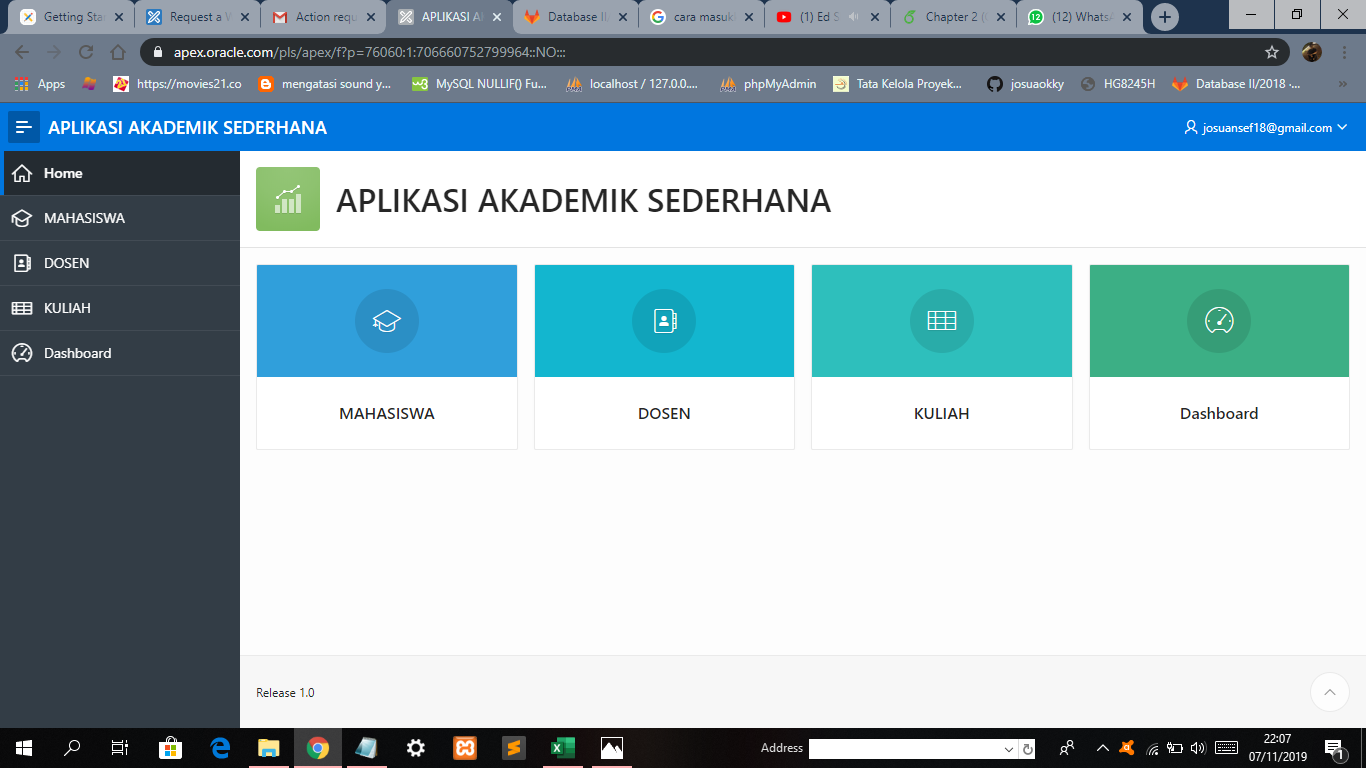
\includegraphics[width=10cm,height=7cm]{figures/32home.png}
\caption{Home Page di Aplikasi}
\label{penanda}
\end{figure}
\end{enumerate}

